\chapter{Feature-based Regularizations}
\label{chapter:regularization}

%\newcommand{\mcL}{\mathcal{L}}
%\newcommand{\vx}{\mathbf{x}}
%\newcommand{\vh}{\mathbf{h}}
%\newcommand{\vy}{\mathbf{y}}
\newcommand{\tableindent}{\,\,\,\,}
\newcommand{\vt}{\mathbf{t}}
%\newcommand{\vyh}{\hat\vy}
\newcommand{\pp}{\,\textit{p.p}}
\newcommand{\std}{$\pm\,$}
\newcommand{\clf}{\textit{clf}}
\newcommand{\gray}[1]{{\color{darkgray}#1}}


\begin{chapabstract}
    Regularization-based methods are powerful approaches to reduce catastrophic
    forgetting, especially in challenging setting such as \ac{CIL} with single-head
    where task identity is not known at test-time. However, they often consider
    only constraining the final probability predictions of the network which falls
    short to forgetting when faced to large amount of tasks. \\
    In this chapter, we propose two methods exploiting explicitly the intermediate
    features to reduce forgetting. The first approach, nicknamed PODNet, aims to
    constrain similar statistics to avoid a representation drift at all levels
    of the network. We show that it scales particularly well on extreme scenarios
    where classes are learned one by one for a long succession of iterations.
    The second approach, named Ghost, pre-emptively reserves
    capacity for future ---yet to be seen--- classes avoiding forgetting before
    it even happens. We pinpoint those classes locations in the representation
    space by estimating their future positions by drawing inspiration from the
    \ac{ZSL} literature.

    The work in this section has led to a publication to a conference paper (PODNet) and a workshop
    paper (Ghost):

    \begin{itemize}
        \item \fullcite{douillard2020podnet}
        \item \fullcite{douillard2020ghost}
    \end{itemize}

\end{chapabstract}
\newpage

\minitoc
\chapterwithfigures{\nameref*{chapter:regularization}}
\chapterwithtables{\nameref*{chapter:regularization}}

\ifthenelse{\boolean{skipRegul}}{\endinput}{}

\section{Introduction}

\ac{CIL}, where each task brings new classes, is among the most challenging setting of \ac{CL}. When
evaluated in single-head, where the task identity is not known at test-time, the majority of the
methods rely on rehearsal learning where a limited amount of old data is replayed. Furthermore, it
is often combined to regularizations that aim to limit forgetting. These regularizations are often a
knowledge distillation \citep{hinton2015knowledge_distillation} that enforces similar probabilities
between the old and current model. First introduced by LwF \citep{li2018lwf}, it has then be used by
multiple seminal papers including iCaRL \citep{rebuffi2017icarl} and WA
\citep{zhao2020weightalignement}. I propose in this chapter two proposed regularization methods to
reduce forgetting. The first one, introduced in \ac{PODNet} \citep{douillard2020podnet} and detailed
in \autoref{sec:podnet}, aims to regularize the statistics shift at the intermediate feature-level
to enforce a consistent representation at multiple levels of the feature extractor across
all steps of the continual training. The second one, nicknamed Ghost \citep{douillard2020ghost} and
described in \autoref{sec:ghost}, on the other hand, avoid pre-emptively forgetting by regularizing the
feature space at locations where future classes are estimated to arrive to.

For both PODNet and Ghost, we will focus on \ac{CIL} where each new task brings new classes. We
propose then to split a dataset into multiple tasks, \ieg{} CIFAR100 50-1 would be 1 task of 50
classes followed by 50 tasks of 1 class each. Following other regularization methods based on the
probabilities, we allow a rehearsal memory storing a limited amount of previous data.

\section{PODNet: reducing forgetting via intermediate feature statistics}
\label{sec:podnet}

\subsection{Related Works}
\label{sec:podnet_related}

We frame our model onto two paradigm: representation learning and regularization-based.

\paragraph{Regularization of the model's output} Regularizations constraining the rate of change of
the weights \citep{kirkpatrick2017ewc} or the gradients \citep{farajtabar2020ogd} have been
proposed. They reduce effectively the forgetting of the feature extractors in a multi-heads setting
where the task identity is known at test-time. However, in the more challenging and realist setting
of single-head, where classes from all tasks, have to be predicted, these methods often barely work
better than a naive finetuning \citep{lesort2019regulshortcomings}. Therefore, I focused on
regularizations applied on a model's output. LwF \citep{li2018lwf} first used the \ac{KD} of
\cite{hinton2015knowledge_distillation}: a KL divergence between the probabilities of the old and
new models. While simple, this loss ---with few variations--- has been used by multiple following
works \citep{rebuffi2017icarl,zhao2020weightalignement}. Few works tried to constrain intermediate
outputs of the model: LwM \citep{dhar2019learning_without_memorizing_gradcam} proposed to minimize
the L2 distance between gradient-based attention maps produced by GradCam
\citep{selvaraju2017gradcam}. M2KD \citep{peng2019m2kd} used a \ac{KD} on both the final predictions
and intermediate predictions from an auxilliary classifier similar to Inception
\citep{szegedy2015inception}. \cite{hou2019ucir} maximizes the cosine similarity between the final
embeddings before the classifier. Finally, \cite{zagoruyko2016distillation_attention}, in the
context of model compression, investigated attention-based distillation for image classifiers, by
pooling the intermediate features of convolutional networks into attention maps, then used in their
distillation losses.

\paragraph{Representation learning} was already implicitly present in
iCaRL~\citep{rebuffi2017icarl}: it introduced the Nearest Mean Exemplars (NME) strategy which
averages the outputs of the deep convolutional network to create a single proxy feature vector per
class that are then used by a nearest-neighbor classifier predict the final classes. Hou et
al.~\citep{hou2019ucir} adopted this method and also introduced another, named CNN, which uses the
output class probabilities to classify incoming samples, freezing (during training) the classifier
weights associated with old classes, and then fine-tuning them on an under-sampled dataset. Hou et
al.~\citep{hou2019ucir}, in the method called here UCIR, made representation learning explicit, by
noticing that the limited memory imposed a severe imbalance on the training samples available for
the old and for the new classes. To overcome that difficulty, they designed a metric-learning model
instead of a classification model. That strategy is often used in few-shot
learning~\citep{gidaris2018fewshot_wo_forgetting} because of its robustness to few data. Because
classical metric architectures require special training sampling (e.g., semi-hard sampling for
triplets), Hou et al. chose instead to redesign the classifier's last layer of their model to use
the cosine similarity~\citep{luo2018cosine_classifier}.


\subsection{Model}
\label{sec:podnet_model}

Our base model is a deep convolutional network $\vyh = g(f(\vx))$, where $\vx$ is the input image,
$\mathbf{y}$ is the output vector of class probabilities, $\vh = f(\vx)$ is the ``feature
extraction'' part of the network (all layers up to the next-to-last), $\vyh = g(\vh)$ is the final
classification layer, and $\vh$ is the final embedding of the network before classification
(\autoref{fig:podnet_model}). The superscript $t$ denotes the model learned at task $t$:$f^{t}$, $g^{t}$,
$\vh^{t}$, etc.

Our strategy is made of two keys components: a distillation loss applied at the intermediate
feature-level, and a local-similarity classifier.

\subsubsection{POD: Pooled Outputs Distillation loss}
\label{sec:podnet_pod}

Constraining the evolution of the weights is crucial to reduce forgetting. Each new task $t$ learns
a new (student) model, whose weights are not only initialized with those of the previous (teacher)
model, but also constrained by a distillation loss. That loss must be carefully balanced to prevent
forgetting (rigidity), while allowing the learning of new classes (plasticity).

To this goal, we propose a set of constraints we call \textbf{Pooled Outputs Distillation (POD)},
applied not only over the final embedding output by $\vh^{t}=f^{t}(\vx)$, but also over the output
of its intermediate layers $\vh^{t}_\ell=f^{t}_\ell(\vx)$ (where by notation overloading
$f^{t}_\ell(\vx)\equiv f^{t}_\ell\circ\ldots\circ f^{t}_1(\vx)$, and thus $f^{t}(\vx)\equiv
    f^{t}_L\ldots\circ f^{t}_\ell\circ\ldots f^{t}_1(\vx)$).

The convolutional layers of the network output tensors $\vh^{t}_{\ell}$ with components
$\vh^{t}_{\ell,c,w,h}$, where $c$ stands for channel (filter), and $w\times h$ for column and row of
the spatial coordinates. The loss used by POD may pool (sum over) one or several of those indexes,
more aggressive poolings (\autoref{fig:podnet_pooling}) providing more freedom, and thus,
plasticity: the lowest possible plasticity imposes an exact similarity between the previous and
current model while higher plasticity relaxes the similarity definition.

Pooling is an important operation in Computer Vision, with a strong theoretical motivation. In the
past, pooling has been introduced to obtain invariant
representations~\citep{lowe1999sift,lazbnik2006spatial_pyramid_matching}. Here, the justification is
similar, but the goal is different: as we will see, the pooled indexes are aggregated in the
proposed loss, allowing \textit{plasticity}. Instead of the model acquiring invariance to the input
image, the desired loss acquires invariance to model evolution, and thus, representation.
%
The proposed pooling-based formalism has two advantages: first, it organizes disparately proposed
distillation losses into a neat, general formalism. Second, as we will see, it allowed us to propose
novel distillation losses, with better plasticity-rigidity compromises. Those topics are explored
next.

\begin{figure}[tb]
    \begin{center}
        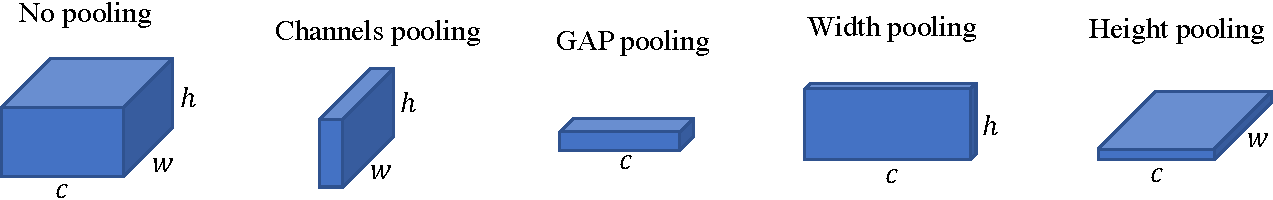
\includegraphics[width=0.90\linewidth]{images/podnet/pooling}
    \end{center}
    \caption{\textbf{Different possible poolings}. The output from a convolutional layer
        $\vh^{t}_{\ell,c,w,h}$ may be pooled (summed over) one or more axes. The resulting loss
        considers only the pooled activations instead of the individual components, allowing more
        plasticity across the pooled axes.}
    \label{fig:podnet_pooling}
\end{figure}

\paragraph{Pooling of convolutional outputs} As explained before, POD constrains the output of each
intermediate convolutional layer $\vh^{t}_{\ell,c,w,h} = f^{t}_\ell(\cdot)$ (in practice, each stage
of a ResNet~\citep{he2016resnet}). As a reminder, $c$ is the channel and $w\times h$ are the spatial
coordinates. All POD variants use the Euclidean distance of $\ell^2$-normalize tensors, here noted
as $\left\Vert\cdot-\cdot\right\Vert$. They differ on the type of pooling applied before that
distance is computed.
%
On one extreme, one can apply no pooling at all, resulting in the most strict loss, the most rigid
constrains, and the lowest plasticity:
%
\begin{equation}
    \mcL_{\text{POD-pixel}}(\vh^{t-1}_\ell, \vh^t_\ell) = \sum_{c=1}^C \sum_{w=1}^{W} \sum_{h=1}^{H} \left\Vert \vh^{t-1}_{\ell,c,w,h} - \vh^t_{\ell,c,w,h} \right\Vert^2\,.
    \label{eq:podnet_pod_pixel}
\end{equation}
%
By pooling the channels, one preserves only the spatial coordinates, resulting in a more permissive
loss, allowing the activations to reorganize across the channels, but penalizing global changes of
those activations across the space,
%
\begin{equation}
    \mcL_{\text{POD-channel}}(\vh^{t-1}_\ell, \vh^t_\ell)  = \sum_{w=1}^{W} \sum_{h=1}^{H} \left\Vert \sum_{c=1}^C \vh^{t-1}_{\ell,c,w,h} - \sum_{c=1}^C \vh^{t}_{\ell,c,w,h} \right\Vert^2\,;
    \label{eq:podnet_pod_channel}
\end{equation}
%
or, contrarily, by pooling the space (equivalent, up to a factor, to a Global Average Pooling), one
preserves \textit{only} the channels:
%
\begin{equation}
    \mcL_{\text{POD-gap}}(\vh^{t-1}_\ell, \vh^t_\ell) = \sum_{c=1}^{C} \left\Vert \sum_{w=1}^{W} \sum_{h=1}^H \vh^{t-1}_{\ell,c,w,h} - \sum_{w=1}^{W} \sum_{h=1}^H \vh^{t}_{\ell,c,w,h} \right\Vert^2\,.
    \label{eq:podnet_pod_gap}
\end{equation}
%
Note that the only difference between the variants is in the position of the summation. For example,
contrast equations \autoref{eq:podnet_pod_pixel} and \ref{eq:podnet_pod_channel}: in the former the
differences are computed between activation pixels, and then totaled; in the latter, first the
channel axis is flattened, then the differences are computed, resulting in a more permissive loss.

We can trade a little plasticity for rigidity, with less aggressive pooling by aggregating
statistics across just one of the spatial dimensions:
%
\begin{equation}
    \mcL_{\text{POD-width}}(\vh^{t-1}_\ell, \vh^t_\ell)  = \sum_{c=1}^{C} \sum_{h=1}^{H} \left\Vert \sum_{w=1}^W \vh^{t-1}_{\ell,c,w,h} - \sum_{w=1}^W \vh^{t}_{\ell,c,w,h} \right\Vert^2\,;
    \label{eq:podnet_pod_width}
\end{equation}
%
or, likewise, for the vertical dimension, resulting in POD-height. Each of those variants measure
the distribution of activation pixels across their respective axis. These two complementary
intermediate statistics can be further combined:
%
\begin{equation}
    \mcL_{\text{POD-spatial}}(\vh^{t-1}_\ell, \vh^t_\ell) = \mcL_{\text{POD-width}}(\vh^{t-1}_\ell, \vh^t_\ell) + \mcL_{\text{POD-height}}(\vh^{t-1}_\ell, \vh^t_\ell)\,.
    \label{eq:podnet_pod_spatial}
\end{equation}
%
$\mcL_{\text{POD-spatial}}$ is minimal when the average statistics over the dataset, on both width
and height axes, are similar for the previous and current model. It brings the right balance between
being too rigid (\autoref{eq:podnet_pod_pixel}) and being too permissive (\autoref{eq:podnet_pod_channel} and
\ref{eq:podnet_pod_gap}).

\label{sec:podnet_pod_flat}
\paragraph{Constraining the final embedding} After the convolutional layers, the network, by design,
flattens the spatial coordinates, and the formalism above needs adjustment, as a summation over $w$
and $h$ is no longer possible. Instead, we set a flat constraint on the final embedding
$\vh^{t} = f^{t}(\vx)$:
%
\begin{equation}
    \mcL_{\text{POD-flat}}(\vh^{t-1}, \vh^t) = \left\Vert \vh^{t-1} - \vh^t \right\Vert^2\,.
    \label{eq:podnet_pod_flat}
\end{equation}

\paragraph{Combining the losses, analysis} The final POD loss combines the two  components:
%
\begin{multline}
    \mcL_\text{POD-final}(\vx) =  \frac{\lambda_{c}}{L-1}\sum_{\ell=1}^{L-1}  \mcL_{\text{POD-spatial}}\left(f^{t-1}_\ell(\vx), f^t_\ell(\vx)\right) + \\[-0.8em]
    \lambda_{f} \mcL_\text{POD-flat}\left(f^{t-1}(\vx), f^t(\vx)\right)\,.
    \label{eq:podnet_pod_final}
\end{multline}
%
The hyperparameters $\lambda_{c}$ and $\lambda_{f}$ are necessary to balance the two terms, due to
the different nature of the intermediate outputs (spatial and flat).

As mentioned, the strategy above generalizes disparate propositions existing both in the literature
of incremental learning, and elsewhere. When $\lambda_{c}=0$, it reduces to the cosine constraint of
\textit{Less-Forget}, proposed by \cite{hou2019ucir} for incremental learning, which constrains only the
final embedding. When $\lambda_{f}=0$ and POD-spatial is replaced by POD-pixel,
it suggests the Perceptual Features loss, proposed for style
transfer~\citep{johnson2016perceptual_losses}. When $\lambda_{f}=0$ and POD-spatial is replaced by
POD-channel, the strategy hints at the loss proposed by \cite{zagoruyko2016distillation_attention}
to allow distillation across different networks, a situation in which the channel pooling responds
to the very practical need to allow the comparison of architectures with different number of
channels.

As we will see in our evaluations of pooling strategies (\autoref{sec:podnet_ablation_pooling}),
what proved optimal was a completely novel idea, POD-spatial, combining two poolings, each of which
flattens one of the spatial coordinates. That relatively rigid strategy (channels and one of the
spatial coordinates are considered in each half of the loss) makes intuitive sense in our context,
which is \textit{small-task} incremental learning, and thus where we expect a slow drift of the
model across a single task.

% ------------------------------------------------------------

\begin{figure}[t]
    \begin{center}
        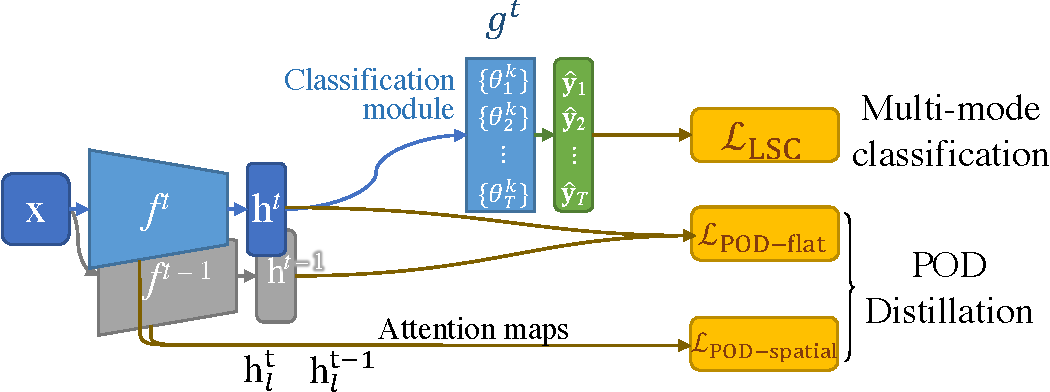
\includegraphics[width=0.8\linewidth]{images/podnet/model}
    \end{center}
    \caption{\textbf{Overview of PODNet}: the distillation loss \ac{POD} prevent excessive model drift by
        constraining intermediate outputs of the \ac{ConvNet} $f$ and the \ac{LSC} classifier $g$ learns a
        more expressive multi-modal representation.}
    \label{fig:podnet_model}
\end{figure}

\subsubsection{Local Similarity Classifier}
\label{sec:podnet_local_classifier}

\cite{hou2019ucir} observed that the class imbalance of incremental learning has
concrete manifestations on the parameters of the final layer on classifiers, namely the weights for
the over-represented (new) classes becoming much larger than those for the underrepresented (old)
classes. To overcome this issue, their method (called here UCIR) $\ell^2$-normalizes both the
weights and the activations, which corresponds to taking the cosine similarity instead of the dot
product. For each class $c$, their last layer becomes
%
\begin{equation}
    \vyh_{c}=\frac{\exp\left(\eta\langle\theta_{c},\vh\rangle\right)}{\sum_{i} \exp \left(\eta\langle\theta_{i}, \vh\rangle\right)}\,,
\end{equation}
%
where $\theta_c$ are the last-layer weights for class $c$, $\eta$ is a learned scaling parameter,
and $\langle\cdot,\cdot\rangle$ is the cosine similarity.

However, this strategy optimizes a \textit{global similarity}: its training objective increases the
similarity between the extracted features and their associated weights. For each class, the
normalized weight vector acts as a \textit{single} proxy~\citep{attias2017proxynca}, towards which
the learning procedure pushes all samples in the class.

We observed that such global strategy is hard to optimize in an incremental setting. To avoid
forgetting, the distillation losses (\autoref{sec:podnet_pod}) tries to keep the final
embedding $\vh$ consistent through time so that the class proxies stay relevant for the classifier.
Unfortunately catastrophic forgetting, while alleviated by current methods, is not solved and thus
the distribution of $\vh$ may change. The cosine classifier is very sensitive to those changes as it
models a unique majority mode through its class proxies.


\paragraph{Local Similarity Classifier} The problem above lead us to amend the classification layer
during training, in order to consider multiple proxies/modes per class. A shift in the distribution
of $\vh$ will have less impact on the classifier as more modes are covered.


Our redesigned classification layer, which we call Local Similarity Classifier (LSC), allows for $K$
multiple proxies/modes during training. Like before, the proxies are a way to interpret the weight
vector in the cosine similarity, thus we allow for $K$ vectors $\theta_{c,k}$ for each class $c$.
The similarity $s_{c,k}$ to each proxy/mode is first computed. An averaged class similarity $\vyh_c$
is the output of the classification layer:
%
\begin{equation}
    s_{c,k} =\frac{\exp\,\langle\theta_{c,k},\vh\rangle}{\sum_{i} \exp\,\langle\theta_{c,i},\vh\rangle}\,, \qquad
    \vyh_c = \sum_{k}s_{c,k}\,\langle\theta_{c,k},\vh\rangle\,.
\end{equation}
%
The multi-proxies classifier optimizes the similarity of each sample to its ground truth class
representation and minimizes all others. A simple cross-entropy loss would work, but we found
empirically that the NCA loss~\citep{goldberger2005nca_loss,attias2017proxynca} converged faster. We
added to the original loss a hinge $[\,\cdot\,]_+$ to keep it bounded, and a small margin $\delta$
to enforce stronger class separation, resulting in the final formulation:
%
\begin{equation}
    \mcL_\text{LSC} = \left[- \log\frac{\exp\left(\eta (\vyh_y - \delta)\right)}{\sum_{i \neq y} \exp \eta \vyh_{i}} \right]_+ \,.
\end{equation}

\paragraph{Weight initialization for new classes} The incremental learning setting imposes detecting
new classes at each new task $t$. New weights $\{\theta_{c,k} \mid \forall c \in C^t_N, \forall k
    \in {1...K}\}$ must be added to predict them. We could initialize them randomly, but the
class-agnostic features of the \ac{ConvNet} $f$, extracted by the model trained so far offer a better
prior. Thus, we employ a generalization of Imprinted Weights~\citep{qi2018imprintedweights}
procedure to multiple modes: for each new class $c$, we extract the features of its training
samples, use a k-means algorithm to split them into $K$ clusters, and use the centroids of those
clusters as initial values for $\theta_{c,k}$. This procedure ensures mode diversity at the
beginning of a new task and resulted in a one percentage point improvement on CIFAR100.

% ------------------------------------------------------------

\subsubsection{Complete model formulation}
\label{sec:podnet_modelsummary}

Our model has the classical structure of a convolutional network $f(\cdot)$ acting as a feature
extractor, and a classifier $g(\cdot)$ producing a score per class. We introduced two innovations to
this model: (1) our main contribution is a novel distillation loss (POD) applied all over the
\ac{ConvNet}, from the spatial features $\vh_\ell$ to the final flat embedding $\vh$; (2) as further
refinement we propose that the classifier learns a multi-modal representation that explicitly keeps
multiple proxy vectors per class, increasing the model expressiveness and thus making it less
sensible to shift in the distribution of $\vh$. The final loss for current model $g^t \circ f^t$,
i.e., the model trained for task $t$, is simply their addition $\mathcal{L}_{\{f^t; g^t\}} =
    \mathcal{L}_\textrm{LSC} + \mathcal{L}_\textrm{POD-final}$. The overall model is displayed in
\autoref{fig:podnet_model}.

\subsection{Experiment results}
\label{sec:podnet_exp}

We compare our technique (\ac{PODNet}) with three state-of-the-art models. Those models are particularly
comparable to ours since they all employ a sample memory with a fixed capacity. Both
iCaRL~\citep{rebuffi2017icarl} and UCIR~\citep{hou2019ucir} use the same inference method
--\ac{NME}, although UCIR also proposes a second inference method
based on the classifier probabilities (called here UCIR-CNN). We evaluate \ac{PODNet} with both inference
methods for a small scale dataset, and the latter for larger scale datasets.
BiC~\citep{wu2019bias_correction}, while not focused on representation learning, is specially
designed to be effective on large scale datasets, and thus provided an interesting baseline.

\paragraph{Datasets} We employ three images datasets --\,extensively used in the literature of
incremental learning\,-- for our experiments: CIFAR100~\citep{krizhevskycifar100},
ImageNet100~\citep{deng2009imagenet,hou2019ucir,wu2019bias_correction}, and
ImageNet1000~\citep{deng2009imagenet}. ImageNet100 is a subset of ImageNet1000 with only 100
classes, randomly sampled from the original 1000.

{\begin{description} \setlength{\parskip}{0pt}
    \item[CIFAR100] contains 32$\times$32-pixel images in 100 classes, with 50k images for training
          and 10k for testing.
    \item[ImageNet100] contains 224$\times$224-pixel images in 100 classes, with $\sim$128k images
          for training and $\sim$5k for testing.
    \item[ImageNet1000] contains 224$\times$224-pixel images in 1000 classes, with $\sim$1.28m
          images for training and $\sim$50k for testing. \end{description}}

\paragraph{Protocol} We validate our model and the compared baselines using the challenging protocol
introduced by \cite{hou2019ucir}: we start by training the models on half the classes
(i.e., 50 for CIFAR100 and ImageNet100, and 500 for ImageNet1000). Then the classes are added
incrementally in steps. We divide the remaining classes equally among the steps, e.g., for CIFAR100
we could have 5 steps of 10 classes or 50 steps of 1 class. Note that a training of 50 steps is
actually made of 51 different tasks: the initial training followed by the incremental steps. Models
are evaluated after each step on \textit{all the classes seen until then}. To facilitate comparison,
the accuracies at the end of each step are averaged into a unique score called \textit{average
    incremental accuracy}~\citep{rebuffi2017icarl}. If not specified otherwise, the average incremental
accuracy is the score reported in all our results.

For CIFAR100 and ImageNet100, we ran all experiments thrice, varying the order of the classes. We
report the averages and standard deviations in tables and graphs. For ImageNet1000, whose models
took much longer to train, we ran each experiment once.

Following \cite{hou2019ucir}, for all datasets, and all compared models, we limit the
memory $M_\textrm{per}$ to 20 images per old class. For results with different memory settings,
refer to \autoref{sec:podnet_robustness}.

\paragraph{Implementation details} For fair comparison, all compared models employ the same \ac{ConvNet}
backbone: ResNet-32 for CIFAR100, and ResNet-18 for ImageNet. We remove the ReLU activation at the
last block of each ResNet end-of-stage to provide a signed input to POD
(\autoref{sec:podnet_pod}). We implemented our method (called here \ac{PODNet}) in
PyTorch~\citep{paszke2017pytorch}.
%
We compare both ours and UCIR's implementation of iCaRL. Results of UCIR come
from the implementation of \cite{hou2019ucir}. We provide their reported results and
also run their code ourselves. We used our implementation of BiC \citep{wu2019bias_correction} in order to compare with the same
backbone.
%
We sample our memory images using \textit{herding selection}~\citep{rebuffi2017icarl} and perform
the inference with two different methods: the \textit{Nearest-Mean-Examplars} (\ac{NME}) proposed for
iCarl, and also adopted on one of the variants of UCIR~\citep{hou2019ucir}, and the ``CNN'' method
introduced for UCIR (see \autoref{sec:podnet_related}).
%
Please see \autoref{sec:appendix_podnet} in the appendix for the full implementation details.


\begin{table*}[t]
    \centering
    \begin{adjustbox}{max width=\textwidth}
        \begin{tabular}{@{}l|cccc@{}}
            \toprule
                                                                         & \multicolumn{4}{|c}{CIFAR100}                                                                            \\
                                                                         & 50 steps                      & 25 steps               & 10 steps               & 5 steps                \\
            \multicolumn{1}{r|}{New classes per step}                    & 1                             & 2                      & 5                      & 10                     \\
            \midrule
            \textit{iCaRL*} \citep{rebuffi2017icarl}                     & ---                           & ---                    & 52.57$\mspace{51mu}$   & 57.17$\mspace{51mu}$   \\
            iCaRL                                                        & 44.20\std0.98                 & 50.60\std1.06          & 53.78\std1.16          & 58.08\std0.59          \\
            BiC \citep{wu2019bias_correction}                            & 47.09\std1.48                 & 48.96\std1.03          & 53.21\std1.01          & 56.86\std0.46          \\
            \textit{UCIR\,{\scriptsize (\ac{NME})}*} \citep{hou2019ucir} & ---                           & ---                    & 60.12$\mspace{51mu}$   & 63.12$\mspace{51mu}$   \\
            UCIR\,{\scriptsize (\ac{NME})}                               & 48.57\std0.37                 & 56.82\std0.19          & 60.83\std0.70          & 63.63\std0.87          \\
            \textit{UCIR\,{\scriptsize (CNN)}*}                          & ---                           & ---                    & 60.18$\mspace{51mu}$   & 63.42$\mspace{51mu}$   \\
            UCIR\,{\scriptsize (CNN)}                                    & 49.30\std0.32                 & 57.57\std0.23          & 61.22\std0.69          & 64.01\std0.91          \\
            PODNet\,{\scriptsize (\ac{NME})}                             & \textbf{61.40\std0.68}        & \textbf{62.71\std1.26} & \textbf{64.03\std1.30} & \textbf{64.48\std1.32} \\
            PODNet\,{\scriptsize (CNN)}                                  & \textbf{57.98\std0.46}        & \textbf{60.72\std1.36} & \textbf{63.19\std1.16} & \textbf{64.83\std0.98} \\
            \bottomrule
        \end{tabular}
    \end{adjustbox}
    \caption{\textbf{CIFAR100 quantitative experiments:} Average incremental accuracy for PODNet \vs state of the art. We run
        experiments three times (random class orders) on CIFAR100 and report averages and
        standard deviations. Models with an asterisk * are reported directly from
        \cite{hou2019ucir}}
    \label{tab:podnet_quantitative_cifar}
\end{table*}

\begin{figure*}[tb]
    \centering
    \begin{subfigure}[b]{0.48\linewidth}
        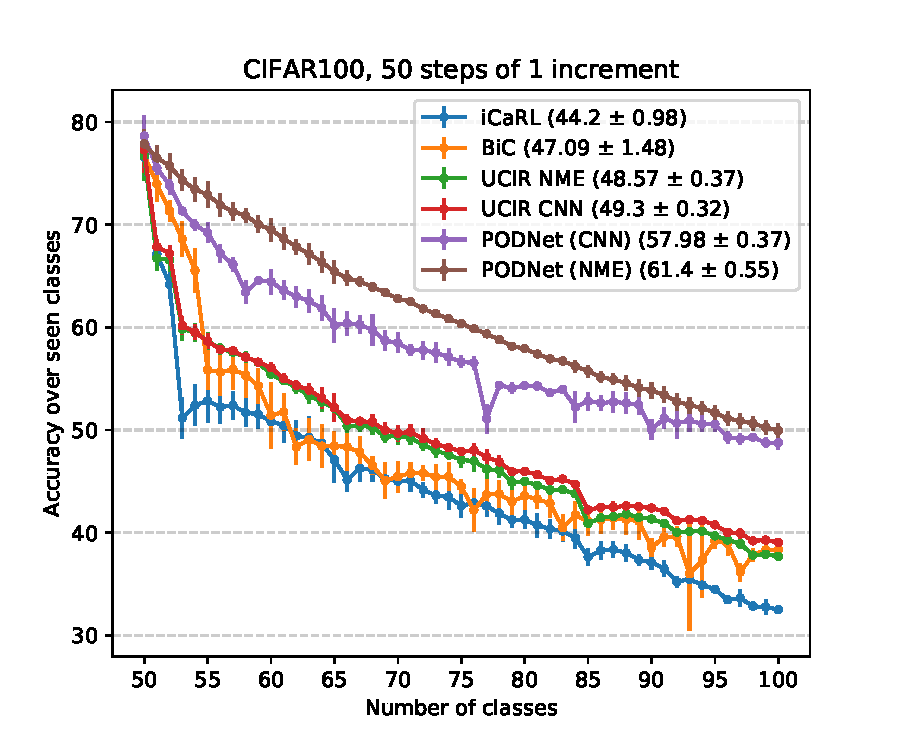
\includegraphics[width=\linewidth]{images/podnet/cifar_inc1}
        \caption{50 steps, 1 class / step}
        \label{fig:cifar_inc1}
    \end{subfigure}
    \hfill
    \begin{subfigure}[b]{0.48\linewidth}
        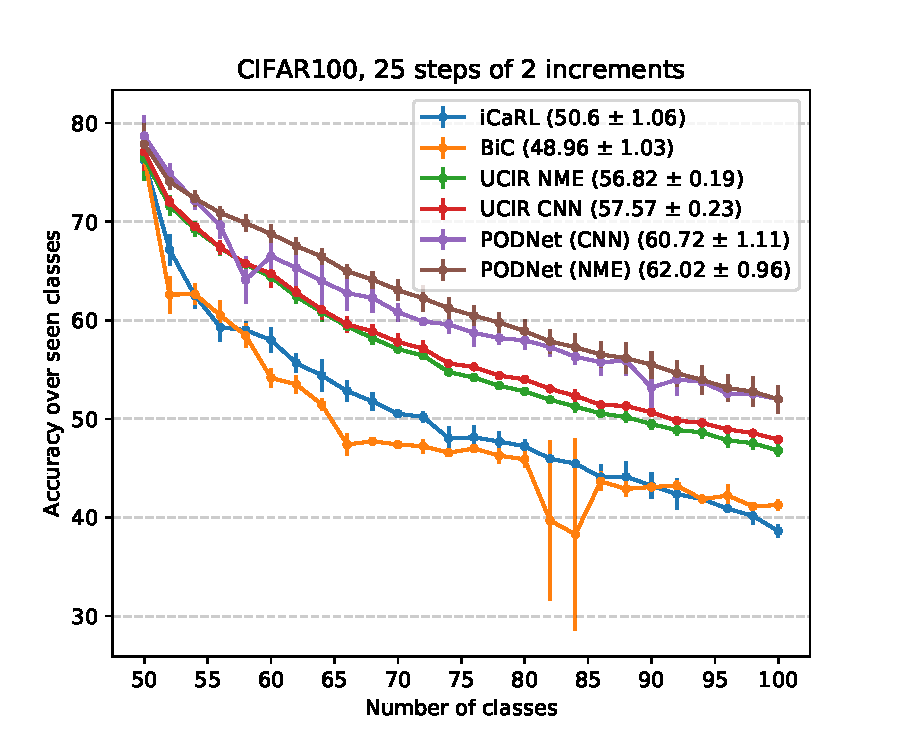
\includegraphics[width=\linewidth]{images/podnet/cifar_inc2}
        \caption{25 steps, 2 classes / step}
        \label{fig:cifar_inc2}
    \end{subfigure}
    \caption{\textbf{Incremental Accuracy on CIFAR100} over three orders for two different step sizes. The legend reports the average incremental accuracy.}
    \label{fig:plots}
\end{figure*}

\begin{table*}[t]
    \centering
    \begin{adjustbox}{max width=\textwidth}
        \begin{tabular}{@{}l|cccc|cc@{}}
            \toprule
                                                                             & \multicolumn{4}{|c|}{ImageNet100} & \multicolumn{2}{c}{Imagenet1000}                                                                                                         \\
            %\cmidrule(l{0pt}r{4pt}){2-4} \cmidrule(l{4pt}r{4pt}){5-7} \cmidrule(l{4pt}r{4pt}){8-9}
                                                                             & 50 steps                          & 25 steps                         & 10 steps                         & 5 steps                          & 10 steps       & 5 steps        \\
            \multicolumn{1}{r|}{New classes per step}                        & 1                                 & 2                                & 5                                & 10                               & 50             & 100            \\
            \midrule
            iCaRL* \scriptsize{\citep{rebuffi2017icarl}}                     & ---                               & ---                              & 59.53                            & 65.04                            & 46.72          & 51.36          \\
            iCaRL                                                            & 54.97                             & 54.56                            & 60.90                            & 65.56                            & ---            & ---            \\
            BiC \scriptsize{\citep{wu2019bias_correction}}                   & 46.49                             & 59.65                            & 65.14                            & 68.97                            & 44.31          & 45.72          \\
            UCIR\,{\scriptsize (\ac{NME})}* \scriptsize{\citep{hou2019ucir}} & ---                               & ---                              & 66.16                            & 68.43                            & 59.92          & 61.56          \\
            UCIR\,{\scriptsize (\ac{NME})}                                   & 55.44                             & 60.81                            & 65.83                            & 69.07                            & ---            & ---            \\
            UCIR\,{\scriptsize (CNN)}*                                       & ---                               & ---                              & 68.09                            & 70.47                            & 61.28          & 64.34          \\
            UCIR\,{\scriptsize (CNN)}                                        & 57.25                             & 62.94                            & 67.82                            & 71.04                            & ---            & ---            \\
            % PODNet\,{\scriptsize (CNN)}                & \textbf{62.48 $\pm$ 0.59} & \textbf{68.31 $\pm$ 2.45} & \textbf{74.33 $\pm$ 0.93} & \textbf{75.54 $\pm$ 0.26} & \textbf{64.13} & \textbf{66.95}\\
            PODNet\,{\scriptsize (CNN)}                                      & \textbf{62.48}                    & \textbf{68.31}                   & \textbf{74.33}                   & \textbf{75.54}                   & \textbf{64.13} & \textbf{66.95} \\

                                                                             & \scriptsize{\textbf{$\pm$ 0.59}}  & \scriptsize{\textbf{$\pm$ 2.45}} & \scriptsize{\textbf{$\pm$ 0.93}} & \scriptsize{\textbf{$\pm$ 0.26}} &                &                \\

            \bottomrule
        \end{tabular}
    \end{adjustbox}
    \caption{\textbf{ImageNet quantitative experiments:} Average incremental accuracy, PODNet \vs
        state of the art. Models with an asterisk * are reported directly from \citet{hou2019ucir}.
        The initial task's sizes are respectively 50 and 500 classes for ImageNet100 and
        ImageNet1000. The remaining classes are learned incrementally.}
    \label{tab:podnet_quantitative_imagenet}
\end{table*}



\subsubsection{Quantitative results}
\label{sec:podnet_quantitative_results}

The comparisons with all the state of the art are tabulated in
\autoref{tab:podnet_quantitative_cifar} for CIFAR100 and \autoref{tab:podnet_quantitative_imagenet}
for ImageNet100 and ImageNet1000. All tables show the average incremental accuracy for each
considered models with various number of steps on the incremental learning run. The ``New classes
per step'' row shows the amount of new classes introduced per task.

\paragraph{CIFAR100} We run our comparisons on 5, 10, 25, and 50 steps with respectively 10, 5, 2,
and 1 classes per step. We created three random class orders to run each experiment thrice,
reporting averages and standard deviations. For CIFAR100 only, we evaluated our model with two
different kinds of inference: \ac{NME} and CNN. With both methods, our model surpasses all previous
state of the art models on all steps. Moreover, our model relative improvement grows as the number
the steps increases, surpassing existing models by 0.82, 2.81, 5.14, and 12.1 percent points (\pp)
for respectively 5, 10, 25, and 50 steps. Larger numbers of steps imply  stronger forgetting; those
results confirm that \ac{PODNet} manages to reduce drastically the said forgetting. While
\ac{PODNet} with \ac{NME} has the largest gain, \ac{PODNet} with CNN also outperforms the previous
state of the art by up to 8.68\pp. See \autoref{fig:podnet_plots} for a plot of the incremental
accuracies on this dataset. In the extreme setting of 50 increments of 1 class
(\autoref{fig:podnet_cifar_inc1}), our model showcases large differences, with slow degradation
(``\textit{gradual forgetting}'' \citep{french1999catastrophicforgetting}) due to forgetting
throughout the run, while the other models show a quick performance collapse (``\textit{catastrophic
    forgetting}'') at the start of the run.

\paragraph{ImageNet100} We run our comparisons on 5, 10, 25, and 50 steps with respectively 10, 5,
2, and 1 classes per step. For both ImageNet100, and ImageNet1000 we report only \ac{PODNet} with CNN, as
the kNN-based \ac{NME} classifier did not generalize as well to larger-scale datasets. With the more
complex images of ImageNet100, our model also outperforms the state of the art on all tested runs,
by up to 6.51\pp.

\paragraph{ImageNet1000} This dataset is the most challenging, with much greater image complexity
than CIFAR100, and ten times the number of classes as ImageNet100. We evaluate the models in 5 and
10 steps, and results confirm the consistent improvement of \ac{PODNet} against existing arts by up to
2.85\pp.

\begin{table*}
    \centering
    \begin{tabular}{@{}lccccc@{}}
        \toprule
        Classifier & POD-flat & POD-spatial & NME            & CNN            \\
        \midrule
        Cosine     &          &             & 40.76          & 37.93          \\
        Cosine     & \OK      &             & 48.03          & 46.73          \\
        Cosine     &          & \OK         & 54.32          & 57.27          \\
        Cosine     & \OK      & \OK         & 56.69          & 55.72          \\
        LSC-CE     & \OK      & \OK         & 59.86          & 57.45          \\
        LSC        &          &             & 41.56          & 40.76          \\
        LSC        & \OK      &             & 53.29          & 52.98          \\
        LSC        &          & \OK         & \textbf{61.42} & 57.64          \\
        LSC        & \OK      & \OK         & 61.40          & \textbf{57.98} \\
        \bottomrule
    \end{tabular}
    \caption{Comparison of the average incremental accuracy on CIFAR100 with 50 steps of the model when disabling parts of the complete \ac{PODNet} loss\\~}
    \label{tab:podnet_ablation_inc}
\end{table*}

\begin{table*}
    \centering
    \begin{tabular}{@{}lcc@{}}
        \toprule
        Loss                                                        & NME            & CNN            \\
        \midrule
        \textit{None}                                               & 53.29          & 52.98          \\
        POD-pixels                                                  & 49.74          & 52.34          \\
        POD-channels                                                & 57.21          & 54.64          \\
        POD-gap                                                     & 58.80          & 55.95          \\
        POD-width                                                   & 60.92          & 57.51          \\
        POD-height                                                  & 60.64          & 57.50          \\
        POD-spatial                                                 & \textbf{61.40} & \textbf{57.98} \\
        \cmidrule{1-3}
        GradCam~\citep{dhar2019learning_without_memorizing_gradcam} & 54.13          & 52.48          \\
        Perceptual Style~\citep{johnson2016perceptual_losses}       & 51.01          & 52.25          \\
        \bottomrule
    \end{tabular}
    \caption{\textbf{Comparison of distillation losses} based on intermediary features. All losses evaluated
        with POD-flat. We report the average incremental accuracy on CIFAR100 with 50 steps.}
    \label{tab:podnet_ablation_perceptual}
\end{table*}

\begin{table*}[!htbp]
    \centering
    \begin{tabular}{@{}lcc@{}}
        \toprule
        Loss                                                        & NME            & CNN            \\
        \midrule
        \textit{None}                                               & 41.56          & 40.76          \\
        POD-pixels                                                  & 42.21          & 40.81          \\
        POD-channels                                                & 55.91          & 50.34          \\
        POD-gap                                                     & 57.25          & 53.87          \\
        POD-width                                                   & 61.25          & 57.51          \\
        POD-height                                                  & 61.24          & 57.50          \\
        POD-spatial                                                 & \textbf{61.42} & \textbf{57.64} \\
        \hdashline
        GradCam~\citep{dhar2019learning_without_memorizing_gradcam} & 41.89          & 42.07          \\
        Perceptual Style~\citep{johnson2016perceptual_losses}       & 41.74          & 40.80          \\
        \bottomrule
    \end{tabular}
    \caption{\textbf{Comparison of distillation losses} based on intermediary features. All losses evaluated
        without POD-flat. We report the average incremental accuracy on CIFAR100 with 50 steps.}
    \label{tab:podnet_ablation_perceptual_noflat}
\end{table*}


\subsubsection{Further analysis \& ablation studies}
\label{sec:podnet_ablation}

\paragraph{Ablation Studies}
Our model has two components: the distillation loss \ac{POD} and the \ac{LSC} classifier. An ablation study
showcasing the contribution of each component is displayed in \autoref{tab:podnet_ablation_inc}: each
additional component improves the model performance. We evaluate every ablation on CIFAR100 with 50
steps of 1 new class each. The reported metric is the average incremental accuracy. The table shows
that our novel method of constraining the whole \ac{ConvNet} is beneficial. Furthermore, applying only
POD-spatial still beats the previous state of the art by a significant margin. Using both
POD-spatial and POD-flat then further increases results with a large gain. We also compare the
results with the Cosine classifier~\citep{luo2018cosine_classifier,hou2019ucir} against the Local
Similarity Classifier (LSC) with NCA loss. Finally, we add LSC-CE: our classifier with multimode
but with a simple cross-entropy loss instead of our modified NCA loss. This version brings to mind
SoftTriple~\citep{qian2019softtriple} and Infinite Mixture
Prototypes~\citep{allen2019infinitemixtureproto}, used in the different context of few-shot
learning.
%The former adds a regularization loss to collapse the multiple proxies into a single one if
%necessary, which we did not find useful in our imbalanced setting of incremental learning.
The latter only considers the closest mode of each class in its class assignment, while \ac{LSC}
considers all modes of a class, thus, taking into account the intra-class variance. That allows \ac{LSC}
to decrease class similarity when intra-class variance is high (which could signal a lack of
confidence in the class).

\label{sec:podnet_ablation_pooling}
\paragraph{Spatial-based distillation} We apply our distillation loss \ac{POD} differently for the flat
final embedding $\vh$ (POD-flat) and the \ac{ConvNet}'s intermediate features maps $\vh_\ell$
(POD-spatial). We designed and evaluated several alternatives for the latter whose results are shown
in \autoref{tab:podnet_ablation_perceptual} and \autoref{tab:podnet_ablation_perceptual_noflat}. Refer to \autoref{sec:podnet_pod}
for their definition. In the first table, all losses are with POD-flat ("\textit{None}" is using only
POD-flat), while in the second table, there is no POD-flat and thus "\textit{None}" has no
distillation loss at all.

Overall, we see that not using pooling results in bad performance (POD-pixels). Our final loss,
POD-spatial, surpasses all others by taking advantages of the statistics aggregated from both
spatial axis. For the sake of completeness we also included losses not designed by us: GradCam
distillation~\citep{dhar2019learning_without_memorizing_gradcam} and Perceptual
Style~\citep{johnson2016perceptual_losses}. The former uses a gradient-based attention while the
later --\,used for style transfer\,-- computes a gram matrix for each channel.

\paragraph{Forgetting and plasticity balance} Forgetting can be drastically reduced by imposing a
high factor on the distillation losses. Unfortunately, it will also degrade the capacity (its
\textit{plasticity}) to learn new classes. When POD-spatial is added on top of POD-flat
(\autoref{tab:podnet_ablation_perceptual}), we manage to increase the oldest classes performance (+7
percentage points) while the newest classes performance were barely reduced (-0.2\pp). Because our
loss POD-spatial constraints only statistics, it is less stringent than a loss based on exact pixels
values as POD-pixel. The latter hurts the newest classes (-2\pp) for a smaller improvement of old
classes (+5\pp). Furthermore, our experiments confirmed that LSC reduced the sensibility of the
model to distribution shift, as the performance it brings was localized on the old classes.

\label{sec:podnet_robustness}
\paragraph{Robustness of our model} While previous results showed that \ac{PODNet} improved significantly
over the state-of-the-arts, we wish here to demonstrate here the robustness of our model to various
factors. In \autoref{tab:podnet_ablation_memorysize}, we compared how \ac{PODNet} behaves against the baseline
when the memory size per class $M_{\text{per}}$ changes: \ac{PODNet} improvements increase as the memory
size decrease, up to a gain of 26.20\pp\ with \ac{NME} (resp. 13.42\pp\ for CNN) with $M_{\text{per}} =
    5$. Notice that by default, the memory size is 20 in \autoref{sec:podnet_quantitative_results}.

We also compared our model against baselines with a more flexible memory $M_{\text{total}} = 2000$
\citep{rebuffi2017icarl,wu2019bias_correction}, and with various initial task size (by default it is
50 on CIFAR100). In the former case (\autoref{tab:podnet_sub_free_memory}), models benefit from a larger
memory per class in the early tasks. In the later case (\autoref{tab:podnet_sub_initialincrement}), models
initialization is worse because of a smaller initial task size. In these settings very different
from \autoref{sec:podnet_quantitative_results}, \ac{PODNet} still outperformed significantly the compared
models, proving the robustness of our model.

\begin{table}[t]
    \centering
    \begin{tabular}{@{}lccccccc@{}}
        \toprule
        $M_{per}$                                                       & 5              & 10             & \textbf{20}    & 50             & 100            & 200            \\
        \midrule
        iCaRL \scriptsize{\citep{rebuffi2017icarl}}                     & 16.44          & 28.57          & 44.20          & 48.29          & 54.10          & 57.82          \\
        BiC \scriptsize{\citep{wu2019bias_correction}}                  & 20.84          & 21.97          & 47.09          & 55.01          & 62.23          & \textbf{67.47} \\
        UCIR\,{\scriptsize (\ac{NME})} \scriptsize{\citep{hou2019ucir}} & 21.81          & 41.92          & 48.57          & 56.09          & 60.31          & 64.24          \\
        UCIR\,{\scriptsize (CNN)}                                       & 22.17          & 42.70          & 49.30          & 57.02          & 61.37          & 65.99          \\
        PODNet\,{\scriptsize (\ac{NME})}                                & \textbf{48.37} & \textbf{57.20} & \textbf{61.40} & \textbf{62.27} & \textbf{63.14} & 63.63          \\
        PODNet\,{\scriptsize (CNN)}                                     & \textbf{35.59} & \textbf{48.54} & \textbf{57.98} & \textbf{63.69} & \textbf{66.48} & \textbf{67.62} \\
        \bottomrule
    \end{tabular}
    \caption{\textbf{Effect of the memory size} per class $M_{per}$ on the models performance.
        Results from CIFAR100 with 50 steps, we report the average incremental accuracy}
    \label{tab:podnet_ablation_memorysize}
\end{table}

\begin{table*}
    \centering
    \begin{tabular}{@{}l|cc@{}}
        \toprule
                                                            & \multicolumn{2}{c}{Nb. steps}                  \\
        \cmidrule{2-3}
        Loss                                                & 50                            & 10             \\
        \midrule
        iCaRL \citep{rebuffi2017icarl}                      & 42.34                         & 56.52          \\
        BiC \citep{wu2019bias_correction}                   & 48.44                         & 55.03          \\
        UCIR\,{\scriptsize (\ac{NME})}\,\citep{hou2019ucir} & 54.08                         & 62.89          \\
        UCIR\,{\scriptsize (CNN)}\,                         & 55.20                         & 63.62          \\
        PODNet\,{\scriptsize (\ac{NME})}                    & \textbf{62.47}                & \textbf{64.60} \\
        PODNet\,{\scriptsize (CNN)}                         & \textbf{61.87}                & \textbf{64.68} \\
        \bottomrule
    \end{tabular}
    \caption{\textbf{Evaluation of an easier memory constraint:} ($M_\mathrm{total} = 2000$)}
    \label{tab:podnet_sub_free_memory}
\end{table*}

\begin{table*}
    \centering
    \begin{tabular}{@{}l|ccccc@{}}
        \toprule
                                                                        & \multicolumn{5}{c}{Initial task size}                                                                     \\
        \cmidrule{2-6}
        Loss                                                            & 10                                    & 20             & 30             & 40             & \textbf{50}    \\
        \midrule
        iCaRL \scriptsize{\citep{rebuffi2017icarl}}                     & 40.97                                 & 41.28          & 43.38          & 44.35          & 44.20          \\
        BiC \scriptsize{\citep{wu2019bias_correction}}                  & 41.58                                 & 40.95          & 42.27          & 45.18          & 47.09          \\
        UCIR\,{\scriptsize (\ac{NME})} \scriptsize{\citep{hou2019ucir}} & 42.33                                 & 40.81          & 46.80          & 46.71          & 48.57          \\
        UCIR\,{\scriptsize (CNN)}                                       & 43.25                                 & 41.69          & 47.85          & 47.51          & 49.30          \\
        PODNet\,{\scriptsize (\ac{NME})}                                & \textbf{45.09}                        & \textbf{49.03} & \textbf{55.30} & \textbf{57.89} & \textbf{61.40} \\
        PODNet\,{\scriptsize (CNN)}                                     & \textbf{44.95}                        & \textbf{47.68} & \textbf{52.88} & \textbf{55.42} & \textbf{57.98} \\
        \bottomrule
    \end{tabular}
    \caption{\textbf{Varying initial task size:} with $M_\mathrm{per} = 20$, and followed by 50 to 90 tasks made of a single class.}
    \label{tab:podnet_sub_initialincrement}
\end{table*}



\section{Ghost: avoid pre-emptively forgetting}
\label{sec:ghost}

Continual learning models contrast with traditional models by approaching a sequence of tasks
incrementally. With limitations (often severe) on the training data they can retain, those models
must avoid catastrophic forgetting of past tasks \cite{robins1995catastrophicforgetting,
    french1999catastrophicforgetting}, while remaining receptive to new tasks. Many approaches exist to
counteract forgetting: keeping a limited amount of training data from previous
tasks~\cite{rebuffi2017icarl,castro2018end_to_end_inc_learn}; learning to generate the training
data~\cite{kemker2018fearnet,shin2017deep_generative_replay}; extending the architecture for new
tasks~\cite{yoon2018dynamically_expandable_networks,li2019learning_to_grow}; using a subnetwork for
each task~\cite{fernando2017path_net,golkar2019neural_pruning, hung2019cpg}; and constraining the
model divergence as it
evolves~\cite{kirkpatrick2017ewc,lopezpaz2017gem,aljundi2018MemoryAwareSynapses,li2018lwf,rebuffi2017icarl,castro2018end_to_end_inc_learn,
    douillard2020podnet}. Those approaches are often complementary.

% Transition and proposition of our data setting
We propose a challenging new setting, \textit{prescient continual learning}, in which the model must
perform well not only for present and past tasks, but also for \textit{future} ones, both avoiding
catastrophic forgetting (using a limited number of training samples for past classes), and giving
the best possible estimates for the future classes (using no training samples at all). To make the
setting possible, the model must know the classes and have some prior information about them.
Indeed, Aljundi et al. \cite{aljundi2019selfless} remark that the ability to make room for future
classes is a key limitation of current continual learning models, and propose a regularization loss
to make the model more “selfless”, explicitly leaving capacity for future classes in the
representation. Han et al. \cite{hanrebuffi2020autodiscovering} proposed a setting where the
training samples from all classes are present from the beginning, but the labels become available
incrementally. In a way, our setting is the inverse: we know which labels we are going to encounter,
but the training data for those labels arrive incrementally. For instance, in many real-world
applications (e.g. fashion product classification), due to budget constraints, models are released
incrementally, with partial classes and training data, despite the classes being known from the
beginning, and being well-characterized by attributes.

% Related work Zeroshot
To address the proposed setting, we take inspiration from zero-shot learning
\cite{lampert2009zeroshot, xian2019awa2}, which allows classifying examples from unseen classes by
combining a vision model with an embedding possessing knowledge about the classes (e.g. a word
embedding \cite{mikolov2013word2vec,pennington2014glove} or an attribute matrix). Although several
approaches exist for zero-shot learning, we will focus on generating a representation for the future
classes \cite{bucher2017zeroshot_gmmn, kumar2018synthesized_zeroshot,
    xian2018feature_generating_zeroshot}. The framework of representation learning will allow us to
integrate continual and zero-shot learning seamlessly, as we advance through the tasks and future
classes become present classes, and then past classes. Moreover, we will be able to use
\textit{ghost features}, predicted features for the future classes, to make room in the
representation space for future classes. All those goals all integrated into a simple, streamlined
model due to a careful construction of the losses.

The contributions of this work are two-fold: (1) we propose a new challenging setting,
\textit{prescient} continual learning, where the model must perform well on past, present, and
\textit{future} classes; (2) we propose our \textit{ghost model} to address that setting,
integrating continual and zero-shot learning into a coherent whole. We evaluate those contributions
in comprehensive experiments, showcasing both the intuitive appeal of our model, and its
performance.


\section{Setting: prescient continual learning}

\label{sec:setting}
\begin{figure}
    \centering
    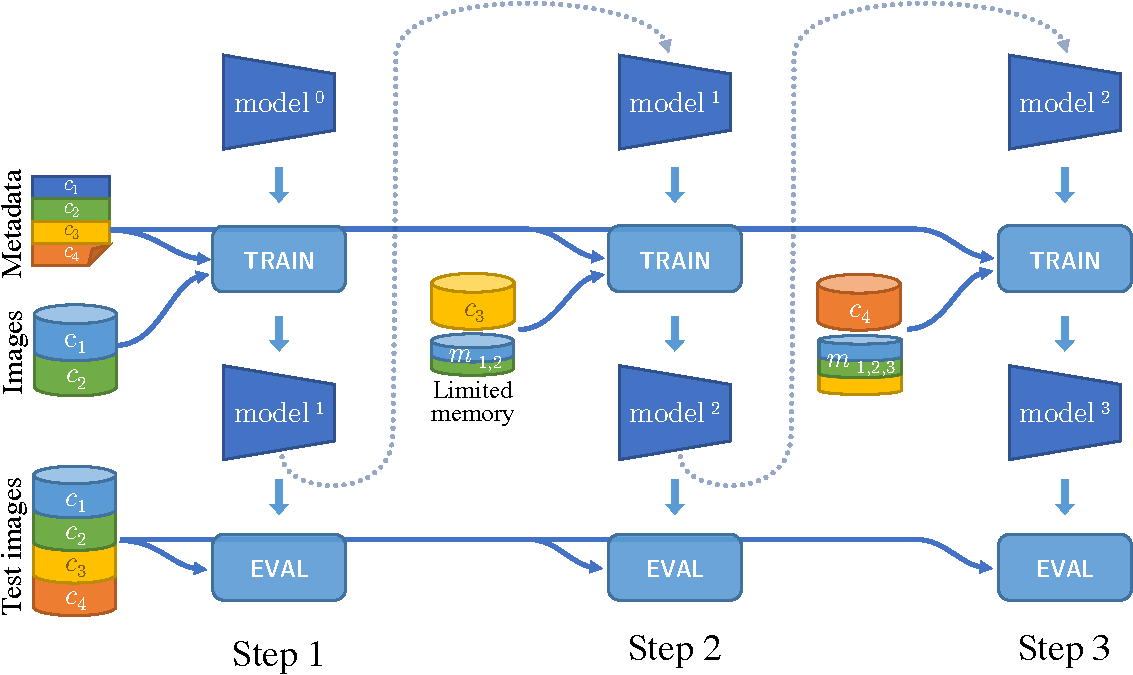
\includegraphics[width=0.7\linewidth]{images/ghost/protocol.pdf}
    \caption{The enriched continual learning setting proposed in this work. At each training task,
        we learn a new set of classes, but the model is evaluated on \textit{all classes} --- past,
        present, and future. The model has to avoid catastrophic forgetting of past classes (using a
        limited number of rehearsal training samples), as well as make a good guess for future classes
        (using no training samples at all).}
    \label{fig:protocol_zeroshot_continual}
\end{figure}


In continual learning, a classifier is trained in multiple steps called \textit{tasks}. Each task
$t\in{1:T}$ comprises a set of new classes $C^t$. The model is evaluated after each task $t$,
traditionally, on all classes seen so far $C^{1:t}$. Our \textit{rehearsal memory} severely limits
the training samples we are allowed to keep from the past classes: following
\cite{hou2019ucir,douillard2020podnet}, we allow a small constant number of samples $s$ per past
class. We must take the maximum advantage from those limited rehearsal data to avoid catastrophic
forgetting.

We propose an enriched experimental setting, prescient continual learning, in which each task is
evaluated on \textit{all classes} $C^{1:T}$: past ($C^{1:t-1}$), present ($C^t$), and future
($C^{t+1:T}$). In that challenging new setting, we must not only avoid the catastrophic forgetting
of past classes (using the limited rehearsal training samples), but also give our best estimates for
future classes (using no training samples at all). That will only be possible if we have some prior
information about the classes, e.g., their hierarchy in a semantic network (like WordNet), an
associated word embedding (like Word2Vec), or an attribute matrix. Such setting is illustrated in
\autoref{fig:protocol_zeroshot_continual}. We will shorthand the set of past and present
classes $C^{1:t}$ as the \textit{seen} classes, and the set of future classes $C^{t+1:T}$ as the
\textit{unseen} classes. We denote individual samples by a superscript $\vx^(i)$, the class
label by a subscript $\vx_c$, and on which parameters a loss is applied by a subscript
$\mcL_\Theta$.

\section{Ghost model}
\label{sec:model}

To address the setting described in the previous section, we propose our \textit{ghost model},
comprising three components: a convolutional feature extractor $f$, a feature generator $g$, and a
classifier $\clf$. The feature extractor is the backbone of the model: it learns to extract a
feature vector from actual samples that can be fed to the classifier. The generator learns the
distribution of the features for all classes, aiming to generate plausible samples of features for
the future classes. The classifier makes the final decision for all classes: past, present, and
future. The classifier is trained on future classes with features sampled from the generator, which
we call \textit{ghost features} (since they must be “hallucinated” from the seen classes and some
prior knowledge about the classes).

All three components are learned continuously throughout the $T$ tasks; we denote the component
learned at task $t$ with a superscript: $f^t$, $g^t$, and $\clf^t$. To avoid catastrophic forgetting
of past classes, we constrain the model's evolution, placing a cost on the divergence between
$f^{t-1}$ and $f^t$. To make the best guess for future classes, we take inspiration from zero-shot
learning, training the classifier with the ghost features. Finally, we adjust the classifier so that
the ghost features “make room” in the representation space for future classes.

The next subsections detail the model, explaining the different terms in the loss that act in
concert to obtain the desired balance.

\subsection{Base model for continual learning}
\label{sec:basemodel}

The base model is a representation-based architecture with a convolutional feature extractor $\vh =
    f(\vx)$ (where $\vx$ is the input image and $\vh$ is the feature vector) and a cosine classifier
$\clf$ \cite{luo2018cosine_classifier, hou2019ucir}, a fully-connected layer with the dot-product
replaced by a cosine similarity:
%
\begin{equation}
    \clf(\vh, \vt)_c = \vyh_c = \frac{\langle \vh, \vt_c \rangle}{\Vert \vh \Vert_2 \Vert \vt_i \Vert_2}\,.
    \label{eq:cosine-classifier}
\end{equation}
%
Remark that $\vt_c$, the parameter vector for the $c$-th class in $\clf$ ($c\in C^{1:t}$), may be
interpreted as a representative or proxy for that class. The classification loss could be either a
cross-entropy loss preceded by softmax activations, or an NCA loss \cite{goldberger2005nca_loss,
    attias2017proxynca, douillard2020podnet}:
%
\begin{equation}
    \mcL^{\text{\tiny{nca}}}_{\Theta_f,\Theta_{\clf}} = \left[- \log\frac{\exp\left(\vyh_y- \delta\right)}{\sum_{c \neq y} \exp \vyh_c} \right]_+ \,.
    \label{eq:nca}
\end{equation}
%
To counteract catastrophic forgetting, we must limit the evolution of the model. We impose — as
usual for continual learning — a distillation loss between the previous model iteration ($t-1$) and
the current one ($t$). We evaluate several distillation losses applied to intermediate and final
outputs of the feature extractor \cite{douillard2020podnet,hou2019ucir} on
\autoref{sec:implementation}. The final loss of the base model is:
%
\begin{equation}
    \mcL = \mcL^{\text{\tiny{nca}}}_{\Theta_f,\Theta_{\clf}} + \lambda_1 \mcL^\text{\tiny{distil}}_{\Theta_f}\,.
    \label{eq:basemodel_loss}
\end{equation}

\subsection{Capacitating ghost model for future classes}

The base model can deal with both present classes (with training samples constrained only by their
availability in the training set)  and past classes (with training samples severely constrained by
the rehearsal memory). As discussed, the introduction of a distillation loss prevents catastrophic
forgetting of the latter. We will now address \textit{future classes}, with \textit{no} training
samples available. First, taking inspiration from zero-shot learning, we will use prior information
about the classes to generate \textit{ghost features}, plausible stand-ins for the unseen future
classes' features. Next, we will adapt the classifier to incorporate those ghost features into the
learning objective seamlessly. The representation learning framework will allow us to integrate the
entire learning apparatus into one coherent loss.

\textbf{Generator} The generative model estimates the distribution of the unseen classes directly
in terms of their features (instead of the input images). For the feature generation to work, we
must have exploitable prior information about the classes, more precisely, we must be able to map
the class labels $c$ into a \textit{class attribute space} that makes semantic sense. The exact way
to perform that mapping will be data-dependent, but most often, either we will have an explicit set
of attributes linked to each class (color, size, material, provenance, etc.), or we will be able to
extract a latent semantic vector, using a technique like Word2vec
\cite{mikolov2013word2vec,pennington2014glove}. The generator learns to link the attributes of the
\textit{seen} classes to the actual feature vectors extracted from the training samples of those
classes. Thus, the first generator training must happen after the feature extractor (its
ground-truth) is learned. The generator is fine-tuned after each task to handle distribution shift.
Next, we ask the generator to draw random samples, using the attributes of the \textit{unseen}
classes, creating counterfeit features that we call \textit{ghost features}. The strategy is
agnostic to the generator model as long as it can be conditioned by class attributes.  At present,
as detailed in \autoref{sec:quantitative}, we choose a Generative Moment Matching Network
\cite{li2015gmmn}: a shallow multi-layer perceptron conditioned by class attributes and a noise
vector trained to minimize the Maximum Mean Discrepancy
\cite{gretton2007twosampleMMD,gretton2012twosampletestMMD}.

\label{sec:generator}

\textbf{Complete classifier.~~} Remind that the parameters  $\{\vt_c\,,\forall c \in C^{1:t}\}$ on
the representation-based classifier (\autoref{eq:cosine-classifier}) may be interpreted as proxies
for the classes $C^{1:t}$. The base model for task $t$ will, thus, learn $|C^{1:t}|$ such proxies,
one for each of the seen classes. To extend the model for the unseen future classes, the complete
classifier will learn $|C^{1:t}| + |C^{t+1:T}|$ proxies, which changes \autoref{eq:nca} to:
%
\begin{equation}
    \mcL^\text{\tiny{nca-ghost}}_{\Theta_f,\Theta_{\clf}} = \left[- \log\frac{\exp\left(\vyh_y - \delta\right)}{\sum_{\substack{c \neq y\\c \in C^{1:t}}} \exp \vyh_{c} + \sum_{\substack{c \neq y\\c \in C^{t+1:T}}} \exp \vyh_{c}} \right]_+ \,.
    \label{eq:nca-ghost}
\end{equation}
%
This classification loss maximizes the similarity $\vyh_y$ (or, conversely, minimizes the distance)
between sample feature $\vh_y$ and correct class proxy $\vt_y$ in the numerator. In the denominator,
the loss pushes away all wrong class proxies, from both seen and unseen (future) classes, by
minimizing the similarities with $\vy_c, \, \forall c \neq y$.

The participation of future classes in the classification loss has two effects. Most obviously, it
allows the model to perform zero-shot-like guesses for those classes during test time. The
representation-learning paradigm allows performing both continual and zero-shot learning seamlessly,
as we advance through the tasks and future classes become present classes, and then past classes.
Less evidently, but vitally important, the learning of proxies for the future classes makes room in
the representation space for those classes, creating effective empty spaces that push away the
actual features of the seen classes (due to the repulsive term in the denominator). As we advance
through training, future classes become present, their ghost placeholders disappear, and they can
neatly fit in the newly vacant region. Such a strategy reduces interference between classes
throughout continual learning, and, as we will see in both visual and quantitative experiments, has
long-range positive effects.

Naturally, the complete classifier has to be trained with samples from all classes. For seen
classes, actual data is available from the training and rehearsal data. For unseen future classes
data is not available, so we employ ghost features sampled from the generator. Note that ghost
features are produced once per task by the generator and are kept fixed for the task duration.
\label{sec:ghost-classifier}

%\begin{figure} \centering \includegraphics[width=\linewidth]{images/zeroshot_training.pdf}
%\caption{The different steps of our training. Starting from the second task, we incorporate our
%Ghost regularization.} \label{fig:zeroshot_training} \end{figure}



\label{sec:svm}
\textbf{Latent-space regularization.~~}
As explained above, our Ghost classification loss minimizes the intra-class distances and maximizes
the inter-class distances. The loss enforces those constraints to all proxies regardless of whether
they represent seen classes or not. We further promote an inter-class separation by optimizing the
latent representation of seen classes to avoid overlapping with the representation of Ghosts. That
loss constrains the features space directly and does not affect the proxies and the intra-class
distances.

We based this regularization loss on SVM \cite{cortes1995svm} for simplicity, but other methods
could have similar behavior. To compute that loss, we learn binary
one-unseen-class-Vs-all-seen-classes SVM classifiers, one for each unseen class. We employ a linear
kernel, since the feature extractor and feature vector dimensionality (512) allows good linear
separation, but more complex kernels could be used. Those SVMs define hyperplanes $\mathbf{w}_c$ and
biases $b_c,\, \forall c \in C^{t+1:T}$, separating each unseen region from the mass of seen
features $\mathbf{h}^{(i)}$ (\autoref{fig:svm_reg}):
%
\begin{equation}
    \mcL^\text{\tiny{svm-reg}}_{\Theta_f} = \frac{1} {N\times |C^{t+1:T}|}\sum_{i=1}^N \sum_{c\in C^{t+1:T}} [\mathbf{w}_c \cdot \mathbf{h}^{(i)} + b_c + \tau]_+\,,
    \label{eq:svm}
\end{equation}
%
where $\mathbf{h}^{(i)}$ are seen features (classes in $C^{1:t}$), $[\,\cdot\,]_+$ the hinge loss,
and $\tau$ an additional margin (higher values of $\tau$ push seen features further away from the
ghost regions, in practice, we set $\tau=1$ to repel beyond the support vectors).

The margin-based regularization of \autoref{eq:svm} refines the ghost classification loss of
\autoref{eq:nca-ghost}. While the latter acts over the classifier conditioning the feature space
indirectly via the action of the class proxies, the former acts directly over the latent/feature
space and the feature extractor backbone that creates it. The computational overhead of training
several SVMs, detailed in the supplementary material, is negligible compared to the total training
time.

\textbf{Complete strategy.~~} All modules and losses fit neatly into the goal of learning
continuously over seen and unseen classes. We train feature extractor (plus classifier) and
generator in alternation. We train the latter to mimic the features of seen classes, and then ask it
to extrapolate to unseen classes (ghost features). Ghost features allow us both to unify seen and
unseen classes into a complete classifier ($\mcL^\text{\tiny{nca-ghost}}$), and to enforce early
allocation in the feature space for unseen classes ($\mcL^\text{\tiny{svm-reg}}$). The complete
loss, in addition to a distillation loss to counter-act catastrophic forgetting
($\mcL^\text{\tiny{distill}}$), is:
%
\begin{equation}
    \mcL = \mcL^\text{\tiny{nca-ghost}}_{\Theta_f,\Theta_{\clf}} + \lambda_1 \mcL^\text{\tiny{distill}}_{\Theta_f} + \lambda_2 \mcL^\text{\tiny{svm-reg}}_{\Theta_f}\,.
\end{equation}
%
An algorithm describing the model's training is provided in the supplementary material.

\begin{figure}
    \centering
    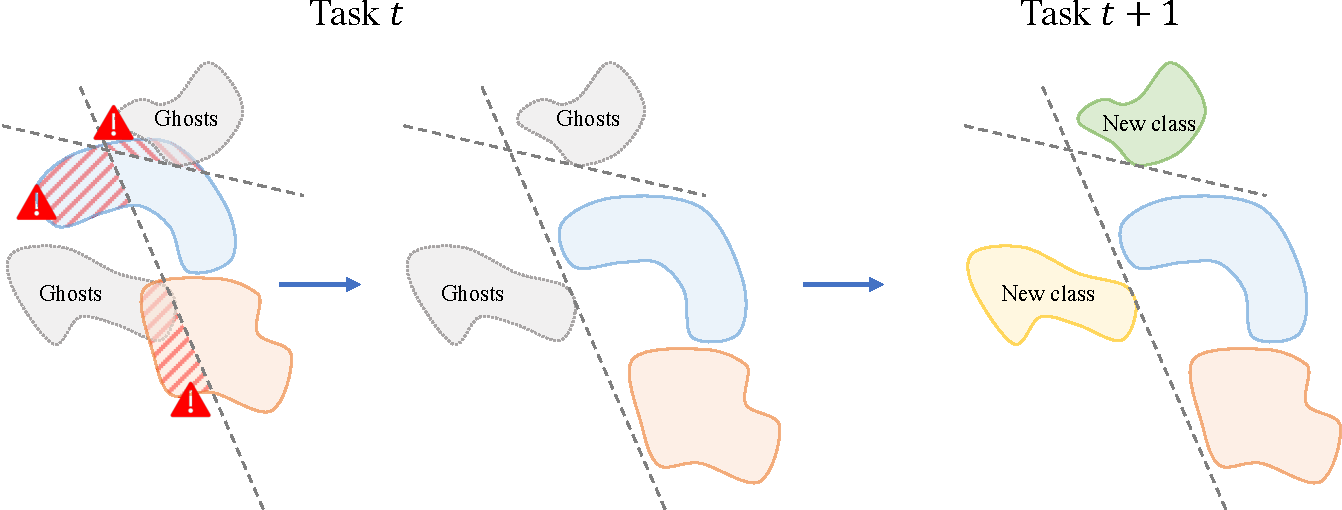
\includegraphics[width=0.7\linewidth]{images/ghost/svm_reg.pdf}
    \caption{Latent-space regularization establishes margin-based one-unseen-class vs. all-seen-classes linear separations. Those separations are employed to directly condition the feature space, creating space for future unseen classes. In the following task, some unseen class will become seen, and may occupy the feature space with less interference.}
    \label{fig:svm_reg}
\end{figure}

\section{Experiments}
\label{sec:implementation}

\subsection{Pictorial experiments}

Before running our full-scale experiments, we will perform a set of experiments with a model that
keeps the main components from the proposed model in a simplified form that will allow us to link
quantitative performances to intuitive visual plots of the feature spaces. For the experiments in
this section we employ the MNIST \cite{lecun2010mnist} dataset, with an initial task of 6 classes
(digits 0 to 5), then two more tasks of two classes each; the feature extractor comprises two
convolutional layers followed by a fully connected layer outputting a feature vector of only two
dimensions — a purposeful choice to allow easy visualization of the feature space. Because MNIST
classes have no attributes, we cannot apply zero-shot learning directly. Instead, we employ the
features of actual images from the future classes instead of samples from the generator — which
corresponds, in some ways, to having a perfectly calibrated generator. Those features are extracted
once per task, and the feature extractor is never trained on unseen classes images. As we will see
in \autoref{tab:generated_vs_real}, integrating the generator in our full-scale model outperforms
using actual extracted features, so that necessary substitution does not exaggerate the abilities of
this small-scale model. The losses used to train the small and the full-scale models are the same,
but the SVM-based regularization was not employed since it made little sense for a 2D latent space.

The 2D feature space allows us to directly visualize the evolution of the feature space as the tasks
progress, without the need for dimensionality reduction techniques that complicate the analysis
(e.g. t-SNE \cite{maaten2008tsne}). \autoref{fig:toy_ghost_weights_3steps} may be interpreted
upfront: as the three tasks progress left-to-right, we see the evolution of the feature space on the
base model (PODNet, on the top branch) and on the proposed model with ghost features (bottom
branch). The base model presents strong overlap between the initial classes, and the later added  8
({\color{orange}orange}) and 9 ({\color{violet}dark purple}). That comes partially from shape
similarities (‘8’ is similar to ‘0’ and ‘5’), partially from continual learning, and results in
severe forgetting of old classes in favor of new ones. The proposed model organizes better the
feature space, which is particularly visible between the second and third steps, where the early
allocation of ghost zones for the future classes (displayed as empty black circles) is prominent.
That better arrangement of the feature space increases the final accuracy from 44 to 66\%, a 22 p.p.
improvement. The small latent space of 2 dimensions explains the low performance for both models; a
model that learns on all classes in one step (\textit{i.e.} not in a continual setting) reaches only
69\% of final accuracy. That said, our model shows a clear improvement both qualitatively in
\autoref{fig:toy_ghost_weights_3steps} and quantitatively. More experiments of this kind can be
found in the supplementary material.

% \subsection{Qualitative assessment} \label{sec:qualitative}
% \subsection{xxxx}https://www.overleaf.com/project/5e986a07010d7400013af43e

\begin{figure}
    \centering
    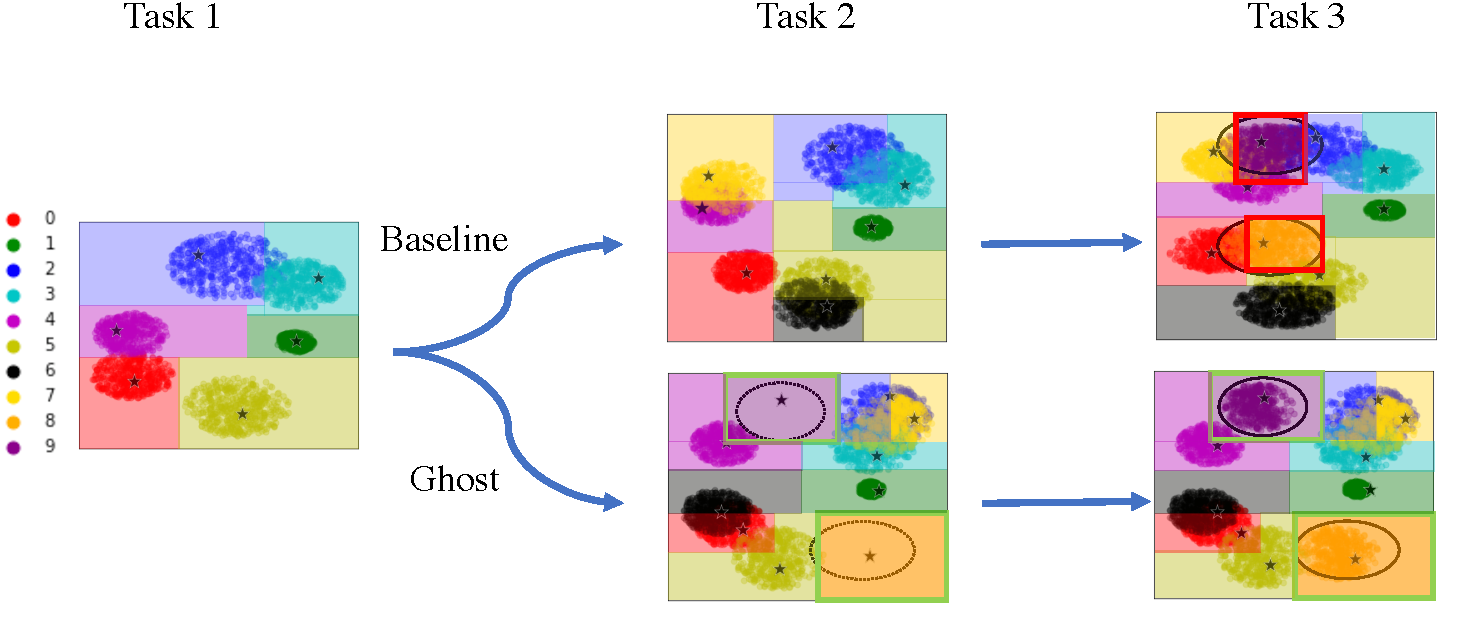
\includegraphics[width=0.8\linewidth]{images/ghost/toy_model_6_2_2.pdf}
    \caption{Small-scale PODNet on MNIST with 3 steps (digits '0' to '5'; then '6' and '7'; then
        '8' and '9') with a features space of only two dimensions. The early incorporation
        of ghost features/proxies in the second task, denoted by dotted circles in the bottom
        row, enforces vacant space for those unseen classes. When filled in the third task
        (last column), there is less interference/overlap with previous classes. Such a
        strategy improves the final accuracy by 22 p.p.}
    \label{fig:toy_ghost_weights_3steps}
\end{figure}

\subsection{Main experiments}
\label{sec:quantitative}

\textbf{Datasets \& Protocols.~~} We perform our experiments on two datasets: AwA2
\cite{xian2019awa2}, with 50 animals categories, each with 85 attributes; and AP\&Y
\cite{farhadi2009apy}, with 32 everyday object classes, each with 64 attributes. We employ two
experimental protocols: one typical for continual learning, following
\cite{hou2019ucir,douillard2020podnet}, starting the first task with half the classes (i.e., 25 for
AwA2, and 16 for aP\&Y), then adding the remaining classes in evenly-sized tasks (5 tasks of 5
classes for AwA2, and 8 tasks of 2 classes for aP\&Y); another inspired from zero-shot learning,
following \cite{xian2019awa2}, starting with a standard selection of classes for each of the
datasets (40 for AwA2, and 20 for aP\&Y), and adding the remaining classes in small increments (5
tasks of 2 classes for AwA2, and 6 tasks of 2 classes for aP\&Y). Our evaluation protocol is akin to
the challenging and realist Generalized Zero-shot Learning \cite{scheirer2013generalizedzeroshot,
    chao2016generalizedzeroshot} protocol  — with no information on whether a sample is from a seen or
unseen class — but harsher, since classes are seen gradually, and training samples for past classes
data are limited by rehearsal memory.

\textbf{Base Models.~~} We evaluate our contributions on top of two different
representation-learning based models, both based on ResNet18 \cite{he2016resnet} feature extractor
backbones (with feature vector size of 512) and cosine classifiers. They differ on the distillation
loss $\mcL_\text{distil}$ employed, the first model (PODNet) using Douillard et al.'s distillation
\cite{douillard2020podnet} constraining the statistics of the intermediate features after each
residual block, and the second (UCIR) using Hou et al.'s distillation \cite{hou2019ucir} enforcing a
cosine constraint on the final flat latent space. The former performs better than the latter, but
both are improved by the innovations proposed in this work. The cosine classifier has a single
proxy/representative per class but could easily be generalized to multiple proxies. Implementation
details are provided in the supplementary material and the code for the entire model will be
released with the final paper.

\textbf{Generator.~~} Following the work of Bucher et al. \cite{bucher2017zeroshot_gmmn} for
zero-shot learning, our generator is a Generative Moment Matching Network (GMMN)~\cite{li2015gmmn}
$g^t(\mathbf{\xi}, \mathbf{E}_c)$, which takes as inputs a Gaussian noise vector $\mathbf{\xi}$ and
a class attributes vector $\mathbf{E}_c$, and outputs a sample from the estimated distribution of
features for a class with the given attributes. In our experiments on AwA2 and AP\&Y, the class
attributes vectors are the average of the attributes for the training samples in the class. For each
task $t$, the feature extractor $f^t$ and the generator $g^t$ are trained to minimize the Maximum
Mean Discrepancy (MMD) \cite{gretton2007twosampleMMD,gretton2012twosampletestMMD} between the actual
features of seen classes $\vh_c = f^t(\vx_c) \, , \forall c \in C^{1:t}$ and their distribution on
the generator $\tilde{\vh}_c = g^t(\mathbf{\xi}, \mathbf{E}_{c}) \,, \forall c \in C^{1:t}$. More
details and figures can be found in the supplementary material.

\begin{table*}
    \caption{Continual Accuracy on AwA2 and aP\&Y for PODNet and UCIR.}
    \label{tab:continual_half}
    \centering
    \begin{tabular}{@{}l|cc|cc@{}}
        \toprule
                                                                                    & \multicolumn{2}{c}{AwA2}                              & \multicolumn{2}{c}{aP\&Y}                                                                                           \\
                                                                                    & \multicolumn{2}{c}{25 classes + 5 $\times$ 5 classes} & \multicolumn{2}{c}{16 classes + 8 $\times$ 2 classes}                                                               \\
                                                                                    & PODNet \cite{douillard2020podnet}                     & UCIR \cite{hou2019ucir}                               & PODNet \cite{douillard2020podnet} & UCIR \cite{hou2019ucir} \\
        \midrule
        Baseline                                                                    & 62.92 \std 0.12                                       & 54.80 \std 0.40                                       & 58.64 \std 0.66                   & 43.42 \std 0.21         \\
        \tableindent+ $\mcL^\text{\tiny{nca-ghost}}$                                & 68.31 \std 0.36                                       & 57.88 \std 0.27                                       & 62.08 \std 0.25                   & 50.23 \std 0.29         \\
        \tableindent+ $\mcL^\text{\tiny{nca-ghost}}$ + $\mcL^\text{\tiny{svm-reg}}$ & 68.46 \std 0.47                                       & 58.08 \std 0.46                                       & 62.73 \std 0.60                   & 50.91 \std 0.56         \\
        %\tableindent+ $\mcL_\text{svm-reg}$ & 63.34 \std 0.13 & 55.34 \std 0.28 & \tbd &\tbd \\
        \bottomrule
    \end{tabular}
\end{table*}

\begin{table*}
    \caption{Final Accuracy on AwA2 and aP\&Y for PODNet and UCIR.}
    \label{tab:final_half}
    \centering
    \begin{tabular}{@{}l|cc|cc@{}}
        \toprule
                                                                                    & \multicolumn{2}{c}{AwA2}                              & \multicolumn{2}{c}{aP\&Y}                                                                                           \\
                                                                                    & \multicolumn{2}{c}{25 classes + 5 $\times$ 5 classes} & \multicolumn{2}{c}{16 classes + 8 $\times$ 2 classes}                                                               \\
                                                                                    & PODNet \cite{douillard2020podnet}                     & UCIR \cite{hou2019ucir}                               & PODNet \cite{douillard2020podnet} & UCIR \cite{hou2019ucir} \\
        \midrule
        Baseline                                                                    & 77.63 \std 0.06                                       & 67.07 \std 0.81                                       & 57.80 \std 0.97                   & 42.23 \std 1.34         \\
        \tableindent+ $\mcL^\text{\tiny{nca-ghost}}$                                & 78.70 \std 0.46                                       & 67.43 \std 0.08                                       & 62.47 \std 0.40                   & 44.17 \std 1.48         \\
        \tableindent+ $\mcL^\text{\tiny{nca-ghost}}$ + $\mcL^\text{\tiny{svm-reg}}$ & 79.08 \std 0.53                                       & 67.53 \std 0.45                                       & 63.30 \std 0.98                   & 45.97 \std 0.26         \\
        %\tableindent+ $\mcL_\text{svm-reg}$ & 78.50 \std 0.10 & 67.0 \std 0.17 & \tbd & \tbd \\
        \bottomrule
    \end{tabular}
\end{table*}


\textbf{Continual Learning with Future Classes.~~}
For continual learning, it is usual to take into account the model's performance as it evolves. We
adapt the traditional average incremental accuracy \cite{rebuffi2017icarl} to take into account
\textit{all} classes, including the future ones, and call that metric \textit{continual accuracy}:
the average of accuracy over all seen classes after each task. The results appear in
\autoref{tab:continual_half}, which shows, for the datasets and protocols explained in the top of
this section, the performance for our two base models \cite{hou2019ucir,douillard2020podnet}, and
the improvements on those base models as we implement our proposed model, with and without the SVM
latent-space regularization refinement. The ability to guess on future class brings large
improvements on both datasets, for both base models. The SVM-based regularization refinement also
improves the results, by up to 0.65 p.p.

\textbf{Final Accuracy.~~} Once we reach the final task, the proposed model ability to guess future
classes provides no advantage due to all classes being now seen. Still, as shown in
\autoref{tab:final_half} — where the metric is simply the accuracy at the final task of each run —
the proposed method outperforms the baselines, due to a better organization of the feature space.
Although the numerical advantages in this table are smaller than in the previous one, these results
are consequential, showing that the ability of the proposed model of incorporating knowledge about
the classes is useful beyond the zero-shot scenario. Again, the SVM-regularization refinement helps
by up to 1.80 p.p.

\begin{figure}
    \centering
    \begin{subfigure}{0.45\linewidth}
        \centering
        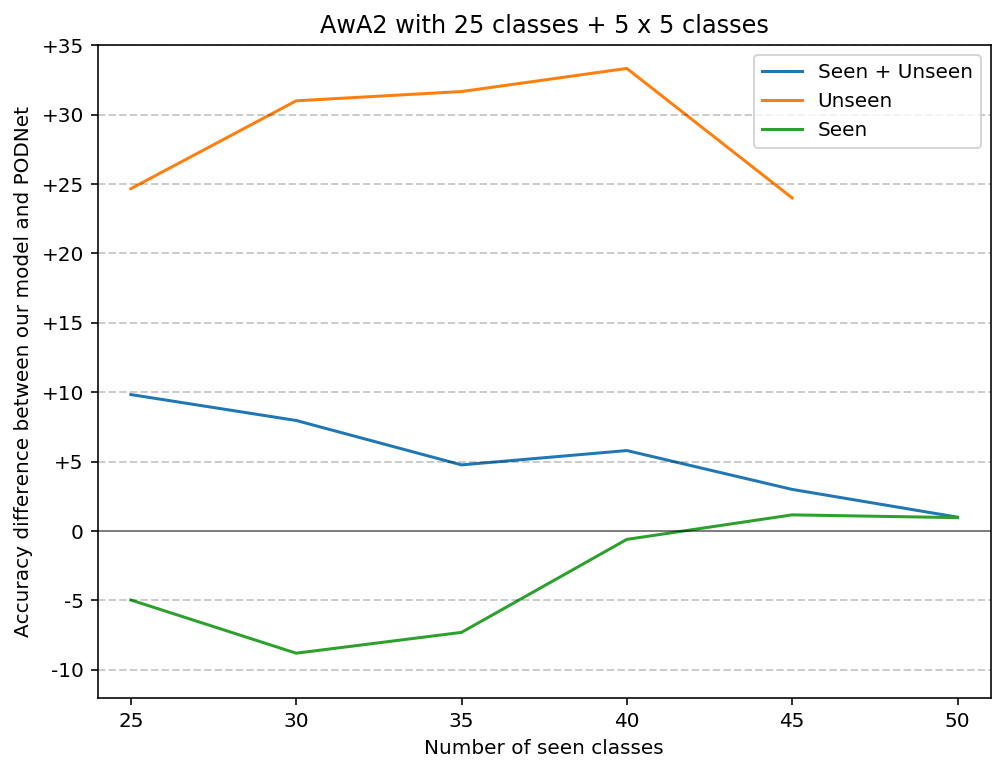
\includegraphics[width=\linewidth]{images/ghost/plot_awa2_25x5x5c_podnet_diff.png}
        \caption{Ghost vs PODNet.}
    \end{subfigure}
    \begin{subfigure}{0.45\linewidth}
        \centering
        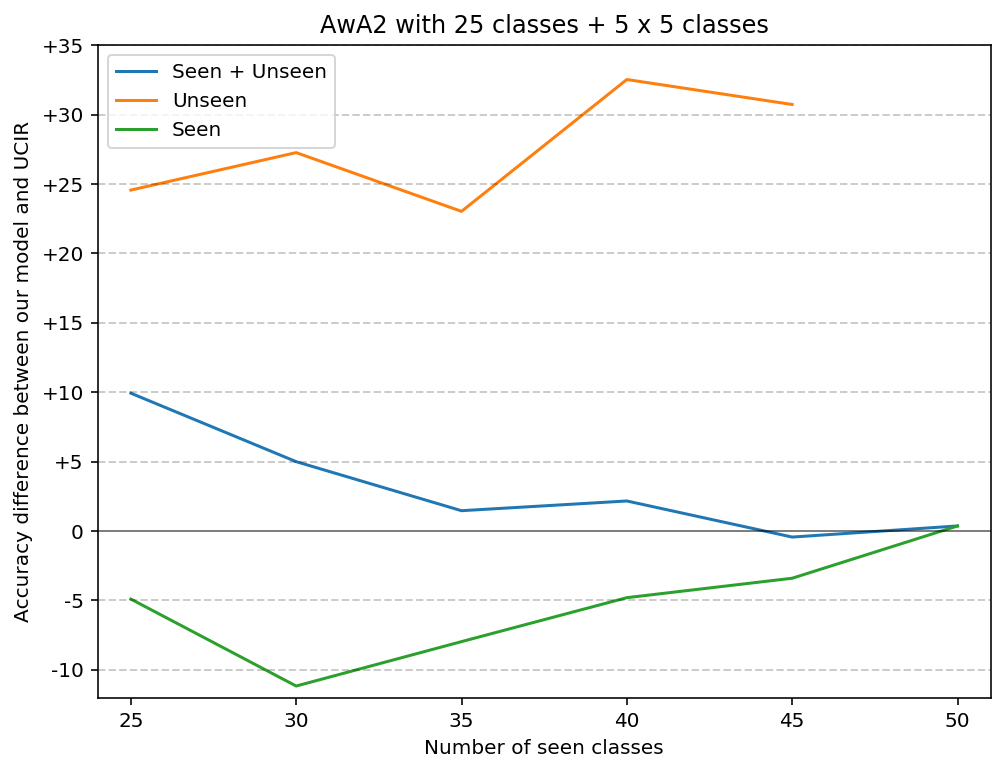
\includegraphics[width=\linewidth]{images/ghost/plot_awa2_25x5x5c_ucir_diff.png}
        \caption{Ghost vs UCIR}
    \end{subfigure}
    \caption{\textbf{Difference of accuracy} over all classes, only seen classes, and only unseen
        classes Ghost model vs base models on AwA2.}
    \label{fig:ghost_plot_awa2_25x5x5c}
\end{figure}


\textbf{Model Evolution.~~} To showcase how the models evolve, plots contrasting the proposed
methods with each base model (PODNet and UCIR) task by task appear in
\autoref{fig:plot_awa2_25x5x5c}. The plots show how, on early tasks, the main advantage of the
proposed model is its ability to guess on the future classes, while on the final task no future
classes remain, but the proposed model still keeps a (more modest, but definitive) advantage.

\begin{table}
    \caption{Further experiments where the initial task size correspond to standard zero-shot seen classes \cite{xian2019awa2}. We report Continual and Final Accuracies for PODNet on AwA2 and aP\&Y.}
    \label{tab:initial_seen}
    \centering
    \begin{tabular}{@{}l|cc|cc@{}}
        \toprule
                                                                                    & \multicolumn{2}{c}{AwA2}                              & \multicolumn{2}{c}{aP\&Y}                                                                 \\
                                                                                    & \multicolumn{2}{c}{40 classes + 5 $\times$ 2 classes} & \multicolumn{2}{c}{20 classes + 6 $\times$ 2 classes}                                     \\

                                                                                    & Continual                                             & Final                                                 & Continual       & Final           \\
        \midrule
        PODNet \cite{douillard2020podnet}                                           & 82.84 $\pm$ 0.10                                      & 84.70 $\pm$ 0.10                                      & 67.57 \std 0.41 & 65.23 \std 0.50 \\
        \tableindent+ $\mcL^\text{\tiny{nca-ghost}}$                                & 84.99 $\pm$ 0.17                                      & 86.57 $\pm$ 0.49                                      & 68.80 \std 0.98 & 67.93 \std 1.24 \\
        \tableindent+ $\mcL^\text{\tiny{nca-ghost}}$ + $\mcL^\text{\tiny{svm-reg}}$ & 84.47 \std 0.15                                       & 85.73 \std 0.40                                       & 69.02 \std 0.46 & 67.97 \std 0.60 \\
        %\tableindent+ $\mcL_\text{svm-reg}$ & 83.58 \std 0.12 & 85.70 \std 0.2° & \tbd & \tbd\\
        \bottomrule
    \end{tabular}
\end{table}


\textbf{Zero-shot-like Initial Task Setting.~~} This set of experiments (\autoref{tab:initial_seen})
is intended for comparison with zero-shot learning benchmarks \cite{xian2019awa2}, which always use
the same split of seen/unseen classes for a given dataset. Our first task in the continual learning
contains the classes defined in zero-shot benchmark as seen, and we learn next, in small increment,
the remaining classes, i.e., those defined in the zero-shot benchmark as unseen. Because the initial
task is larger than previously, fewer future classes remain, and the base models have better
performance. Still, the proposed method improves both base methods in both datasets significantly.
The setting proposed is different than the — markedly less challenging — setting appearing in
Kankuekul et al.\cite{kankuekul2012onlineincrementalzeroshot} and Xue et
al.\cite{xue2017incrementalzeroshot}, where the set of unseen classes is fixed, and only more seen
classes are added incrementally, without any sample limitations given by rehearsal memory.

% We completed further experiments with a different task setting. Instead of an initial task of half
% the classes, as \cite{hou2019ucir,douillard2020podnet}, we initial train the model on Zeroshot's
% seen classes: usual Zeroshot Learning benchmarks uses the same split seen/unseen. In our Continual
% Zeroshot Learning, we pick as initial task what benchmarks defines as "seen". Then initial tasks
% are of larger size than previous setting (\autoref{tab:continual_half,tab:final_half}), thus

\begin{table*}
    \centering
    \begin{adjustbox}{max width=\textwidth}
        \begin{tabular}{@{}l|cc|cc@{}}
            \toprule
                                          & \multicolumn{2}{c}{AwA2}                              & \multicolumn{2}{c}{aP\&Y }                                                                              \\
                                          & \multicolumn{2}{c}{25 classes + 5 $\times$ 5 classes} & \multicolumn{2}{c}{16 classes + 8 $\times$ 2 classes}                                                   \\
                                          & Continual                                             & Final                                                 & Continual              & Final                  \\
            \midrule
            %\textit{None} & &  & \OK & 62.92 \std 0.12 & 77.63 \std 0.06 & 58.64 \std 0.66 & 57.80 \std 0.97\\
            Our model                     & 68.46 \std 0.47                                       & 79.08 \std 0.53                                       & 62.73 \std 0.60        & 63.30 \std 0.98        \\
            \tableindent w/ real features & 67.65 \std 0.50                                       & 78.83 \std 0.31                                       & 61.88 \std 0.52        & 61.70 \std 0.26        \\
            \gray{Partial oracle}         & \gray{72.94 \std 0.25}                                & \gray{84.60 \std 0.28}                                & \gray{63.81 \std 0.29} & \gray{68.03 \std 1.42} \\
            \gray{Full oracle}            & ---                                                   & \gray{95.40 \std 0.02}                                & ---                    & \gray{97.40 \std 0.30} \\
            \bottomrule
        \end{tabular}
    \end{adjustbox}
    \caption{\textbf{Comparison of generated ghost features vs. actual features} extracted from future classes'\,samples with PODNet on AwA2 and aP\&Y.}
    \label{tab:ghost_generated_vs_real}
\end{table*}


\textbf{Generator Validation.~~} The generator approximates the feature extractor for the unseen
future classes. To validate its effectiveness, we replace the generated features by the actual
features from the future images. This form of “cheating”, of course, is not possible in
\textit{actual} real-world scenarios, but serves as a metric. \autoref{tab:generated_vs_real} shows
the comparison, with the surprising result that generated features performed better than the actual
features from samples (respectively first and second row). Note that the latter are extracted once
per task. We hypothesize it explains the score difference because the features extractor was never
adapted for the unseen classes distribution. The “oracle” experiments in the third and fourth row in
\autoref{tab:generated_vs_real} establish an upper bound for what we could achieve by ”cheating”
around the experimental protocol restrictions. The partial oracle from third row is the same model
as the second row, fine-tuning the feature extractor with samples coming from the future. The full
oracle of the fourth line uses all images from all classes unrestrictedly in a single task. Despite
the partial oracle had full access to real future data, we stress that our model's performance with
generated future data is close to this upper bound.
%Both oracles have obviously better performances that our method, but we stress that our method is
%close to the partial oracle with a difference smaller than 5 p.p. (in other words, it follows a
%vanilla supervised protocol instead of a continual learning one)

%A visual analysis of the ghost features vs. actual features (\autoref{fig:tsne_projection_ghost})
%shows that the ghost features are, in general, well-calibrated in terms of the rough region of
%space occupied, but have a much smaller variance than actual features from samples of unseen
%classes. That smaller variance/diversity may end up better working to regularize the feature space,
%acting as ``archetypal'' class examples.

% We hypothesise that this can be explained by the intra-class diversity, as seen in
% \autoref{fig:tsne_projection_ghost}, which is high for real features while low for generated
% features. Recall that for ``\textit{real}'', the features extractor was never trained on those
% unseen classes, the latent space it produced it thus uncertain.

%\input{tables/quantitative_pod} \input{tables/qualitative_podflat}

%We also inspected the features we generated for a AwA2, a larger-scale dataset.
%\autoref{fig:tsne_projection_ghost} showcases a t-SNE 2d projection of the latent space for real
%and generated features. \autoref{fig:tsne_seen} contains the features of \textit{seen} classes, the
%generator was trained to approximate those. In \autoref{fig:tsne_unseen}, the generator extrapolate
%its knowledge to \textit{unseen} classes. As remarked by others \cite{ravuri2019accongan},
%generative models don't yet produce the most realistic images/features. However in a setting as
%constrained as ours, where unseen classes are totally nonexistent, generating them provide a much
%needed insights of the future.

\section{Conclusion}

In this work, we introduced prescient continual learning, a new challenging setting for continual
learning, where the model trains on a sequence of tasks, each introducing new classes, but has
access to prior information about the classes. Although we give the model awareness of future
classes, we also test it on all classes: past, present, and future, resulting in a more challenging
setting. We proposed ghost model, first of its kind, which uses the paradigm of representation
learning to incorporate capabilities of zero-shot learning into the continual learning model in a
seamless way. We refined that model with a novel SVM-based regularization loss acting over the
feature space to reinforce exclusion zones, reserved for future classes. Finally, we established, in
extensive quantitative and qualitative experiments, the advantage of the proposed model over two
base models.


\section{Conclusion}

